\documentclass[sigconf]{acmart}

\usepackage{algorithm}
\usepackage{algorithmic}
\usepackage{subcaption}
\usepackage{listings}
\lstset{literate=%
    {Ö}{{\"O}}1
    {Ä}{{\"A}}1
    {Ü}{{\"U}}1
    {ß}{{\ss}}1
    {ü}{{\"u}}1
    {ä}{{\"a}}1
    {ö}{{\"o}}1
    {~}{{\textasciitilde}}1
}
\lstset{
    numbers=left, % Line numbers on the left
    numberstyle=\small,
    stepnumber=1,
    basicstyle=\ttfamily,
    frame=single,
    breaklines=true,
    breakatwhitespace=true,
}
\AtBeginDocument{%
  \providecommand\BibTeX{{%
    Bib\TeX}}}
\setcopyright{acmlicensed}
\copyrightyear{2024}
\acmYear{2024}
\acmDOI{XXXXXXX.XXXXXXX}
\acmConference[SIGMOD '24]{Proceedings of the 2024 International Conference on Management of Data}{June 11--16, 2024}{Santiago, Chile}
\acmISBN{978-1-4503-XXXX-X/24/06}

\begin{document}
\title{Reducing Destatis Excel Files by 99.9\%: Introducing 'Excel Shrink'}

\author{Alexander Aue-Johr}
\email{alexander.aue@thuenen.de}
\orcid{0009-0001-8683-3630}
\affiliation{%
  \institution{Institute of Rural Studies, Johann Heinrich von Thünen Institute}
  \city{Braunschweig}
  \country{Germany}
}

\renewcommand{\shortauthors}{Aue-Johr, A.}

\begin{abstract}
The German Federal Statistical Office (Destatis) publishes a multitude of Excel sheets containing statistical data. However, these files are often significantly larger than necessary due to unused cell formats, empty cells, and other inefficiencies, leading to increased storage requirements and slower data processing. In this paper, we introduce \textit{Excel Shrink}, an open-source tool that reduces the file size of these Excel sheets by up to 99.9\%. We analyze the root causes of the excessive file sizes, describe our method for identifying and eliminating redundant content, and compare our tool with existing solutions. Our evaluation on a comprehensive dataset of Destatis Excel files demonstrates substantial improvements in file size reduction without altering the visual appearance of the spreadsheets.
\end{abstract}

\begin{CCSXML}
<ccs2012>
<concept>
<concept_id>10002951.10002952.10003190</concept_id>
<concept_desc>Information systems~Database management system engines</concept_desc>
<concept_significance>500</concept_significance>
</concept>
<concept>
<concept_id>10010405.10010455.10010460</concept_id>
<concept_desc>Applied computing~Document management and text processing</concept_desc>
<concept_significance>300</concept_significance>
</concept>
<concept>
<concept_id>10002951.10002952.10003197</concept_id>
<concept_desc>Information systems~Query languages</concept_desc>
<concept_significance>100</concept_significance>
</concept>
</ccs2012>
\end{CCSXML}

\ccsdesc[500]{Information systems~Database management system engines}
\ccsdesc[300]{Applied computing~Document management and text processing}
\ccsdesc[100]{Information systems~Query languages}

\keywords{Excel file optimization, data cleaning, open data, file size reduction, data preprocessing}

\begin{teaserfigure}
  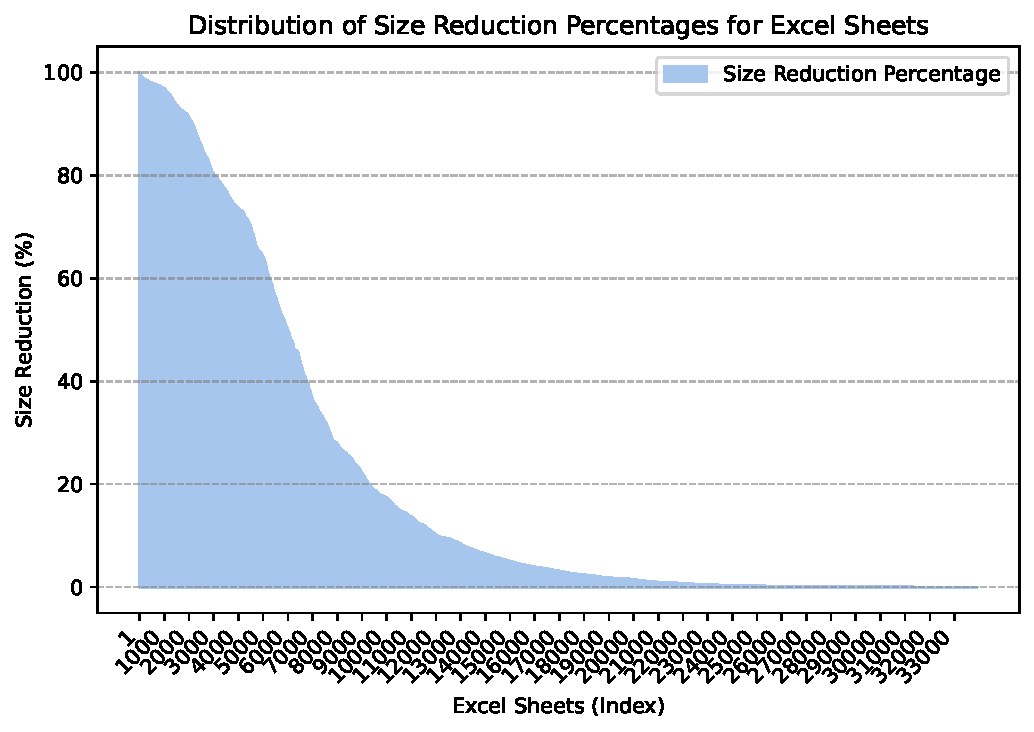
\includegraphics[width=\textwidth]{images/charts/distribution_of_size_reduction.pdf}
  \caption{Distribution of Size Reduction Percentages for Excel Sheets}
  \Description{Histogram showing the distribution of size reduction percentages for Excel sheets processed by Excel Shrink.}
  \label{fig:teaser}
\end{teaserfigure}

\maketitle

\section{Introduction}

Excel files are widely used as a data exchange format due to their versatility and user-friendly interface. However, unlike simpler formats such as CSV, where the file content directly corresponds to what the user sees, Excel files store data in a complex structure involving multiple XML files within a compressed archive. While this structure allows for advanced features and data representation, it can also lead to significant inefficiencies, especially when files contain unnecessary formatting or empty cells.

In our work with Excel files provided by the German Federal Statistical Office (Destatis), we observed that many of these files were excessively large, leading to long loading times and increased processing overhead. Upon investigation, we found that the actual amount of meaningful data was relatively small, and the large file sizes were primarily due to unnecessary definitions of columns, rows, and cells that did not contain any data or contributed to the spreadsheet's appearance.

To address this issue, we developed \textit{Excel Shrink}, an open-source tool designed to analyze and reduce the file sizes of Excel sheets by eliminating redundant content. In some cases, we achieved reductions of up to 99.9\% in file size. In this paper, we present our methodology for identifying and removing unnecessary elements from Excel files, analyze the patterns leading to bloated file sizes, and compare our tool with existing solutions.

Our contributions are as follows:

\begin{itemize}
    \item We identify the common practices and issues that lead to unnecessarily large Excel files, particularly in the context of Destatis data.
    \item We develop \textit{Excel Shrink}, an open-source tool that efficiently reduces Excel file sizes without altering the visual presentation of the data.
    \item We evaluate our tool on a comprehensive dataset of Destatis Excel files, demonstrating significant improvements over existing solutions.
\end{itemize}

The rest of the paper is organized as follows. Section~\ref{sec:related_work} discusses related work. Section~\ref{sec:methodology} describes our approach to analyzing and reducing Excel file sizes. Section~\ref{sec:evaluation} presents our experimental results. Section~\ref{sec:conclusion} concludes the paper.

\section{Related Work}
\label{sec:related_work}

Several tools and methods have been developed to optimize Excel files and reduce their sizes. Commercial software like \textit{NXPowerLite Desktop} \cite{neuxpower2024nxpowerlite} offers file compression and optimization features, including the removal of unused cells and formatting. Microsoft provides the \textit{Inquire} Add-in for Excel \cite{inquire_addin}, which helps users analyze and clean up workbooks by detecting issues like hidden data and unused cells.

However, these tools often have limitations. They may not fully remove all redundant content, may require manual intervention, or may not be suitable for batch processing large numbers of files. Additionally, some features are only available in specific versions of Excel, limiting accessibility.

Research on spreadsheet optimization has also explored methods for detecting and removing redundant data \cite{spreadsheet_reduction}. Techniques include analyzing the workbook's structure, identifying patterns of unnecessary formatting, and automating the cleanup process.

Our work differs by focusing specifically on the challenges presented by large-scale, publicly available statistical data from Destatis. We provide an open-source solution that can process large batches of Excel files efficiently, addressing specific issues not fully resolved by existing tools.

\section{Methodology}
\label{sec:methodology}

In this section, we describe our approach to analyzing the Excel files from Destatis, identifying the causes of excessive file sizes, and developing a tool to eliminate unnecessary content.

\subsection{Understanding Excel File Structure}

An Excel file (.xlsx) is essentially a ZIP archive containing multiple XML files that define the workbook's structure, styles, shared strings, and data. Excel uses mechanisms like shared strings to store recurring text centrally, reducing redundancy. However, issues arise when users inadvertently introduce unnecessary formatting or data definitions.

Common practices that contribute to bloated file sizes include:

\begin{itemize}
    \item Applying formats to entire rows or columns beyond the used range.
    \item Duplicating worksheets and not removing excess formatting.
    \item Leaving behind hidden or empty cells with formatting.
    \item Including cells with whitespace or non-visible characters.
\end{itemize}

These practices lead to large XML files defining cells, rows, and columns that are not actually in use.

\subsection{Scraping Destatis Data}

To analyze the extent of the issue, we scraped all available Excel files from the Destatis website. Since Destatis does not provide an API for accessing its publications, we developed a web scraper that navigates the website, respects the site's crawl-delay policy, and downloads the Excel files.

Our scraper:

\begin{itemize}
    \item Searches for publications containing Excel attachments.
    \item Handles pagination and filters to minimize the number of requests.
    \item Caches downloaded URLs to avoid duplicates.
    \item Waits 30 seconds between requests, as specified in Destatis' robots.txt.
\end{itemize}

Algorithm~\ref{alg:scraper} outlines the scraping process.

\begin{algorithm}
  \caption{Web Scraping and Downloading Excel Files with Caching}
  \label{alg:scraper}
  \begin{algorithmic}
      \STATE \textbf{Input:} Base URL $B$, download folder $D$, cache file $C$
      \STATE Initialize cached URLs $U$ from $C$
      \FOR{each year $y$ in range}
          \STATE Construct search URL $S$ with year $y$
          \WHILE{more pages to fetch}
              \STATE Fetch page $P$ from $S$
              \STATE Extract Excel links $L$ from $P$
              \FOR{each link $l$ in $L$}
                  \IF{$l \notin U$}
                      \STATE Download file from $l$ to $D$
                      \STATE Add $l$ to $U$ and update $C$
                  \ENDIF
              \ENDFOR
              \STATE Update $S$ to next page URL
          \ENDWHILE
      \ENDFOR
  \end{algorithmic}
\end{algorithm}

\subsection{Analyzing and Reducing File Sizes}

We developed \textit{Excel Shrink}, a tool that processes Excel files and removes unnecessary content without altering the visible data or formatting. The tool performs the following steps:

\begin{enumerate}
    \item Parses the workbook and identifies the used range of cells.
    \item Removes definitions of empty cells, rows, and columns outside the used range.
    \item Cleans up shared strings that are not referenced.
    \item Ensures that cell styles and formats are preserved for visible data.
    \item Repackages the Excel file with the reduced XML content.
\end{enumerate}

Key challenges include handling cells with invisible content (e.g., whitespace), preserving formatting that affects the appearance, and maintaining the integrity of the XML structure to prevent corruption.

\subsection{Handling Special Cases}

Certain issues required special attention:

\paragraph{Whitespace Cells}

Cells containing only whitespace can be invisible but still consume space due to shared string references. We detect and remove such cells by checking the shared strings and ensuring that their removal does not affect the spreadsheet's appearance.

\paragraph{Empty Columns and Rows}

Definitions of columns and rows that do not contain data or affect formatting are removed. However, we ensure that any custom widths or heights that are visually significant are preserved.

\paragraph{Cell Borders and Styles}

Cells with borders or styles that contribute to the spreadsheet's layout are retained. We analyze the cell style definitions to determine whether a cell's formatting is necessary for the visual presentation.

\section{Evaluation}
\label{sec:evaluation}

We evaluated \textit{Excel Shrink} on the dataset of 1,182 Excel files downloaded from Destatis. Our evaluation focuses on file size reduction and preservation of the spreadsheet's visual appearance.

\subsection{File Size Reduction}

Figure~\ref{fig:size-reduction-chart} shows the distribution of size reduction percentages across the processed Excel sheets. The results demonstrate that our tool achieved significant reductions:

\begin{itemize}
    \item For 17 sheets, file sizes were reduced by over 99.9\%.
    \item 95 sheets saw reductions over 99\%.
    \item 453 sheets had reductions over 98\%.
\end{itemize}

Table~\ref{tab:top_size_reduction} lists the top 10 sheets with the highest size reductions.

\begin{table}[htbp]
  \caption{Top Size Reduction Results}
  \label{tab:top_size_reduction}
  \centering 
  \begin{tabular}{lrrr}
    \toprule
    \textbf{File} & \textbf{Original Size (KB)} & \textbf{Reduced Size (KB)} & \textbf{Reduction (\%)} \\
    \midrule
    verkehrsunfaelle-zeitreihen.xlsx (Sheet: Technisch\_bedingte\_Leerseit) & 52,367 & 19 & 99.96 \\
    verkehrsunfaelle-zeitreihen.xlsx (Sheet: 3.1\_(7)) & 77,556 & 30 & 99.96 \\
    statistischer-bericht-kostenstruktur-med-bereich.xlsx (Sheet: 52571-10) & 30,630 & 21 & 99.93 \\
    % Add more entries as needed
    \bottomrule
  \end{tabular}
\end{table}

\subsection{Preservation of Visual Appearance}

We manually inspected a sample of the processed Excel sheets to ensure that the visual appearance remained unchanged. Our tool successfully preserved the formatting, styles, and layout of the spreadsheets, with no noticeable differences to the end user.

\subsection{Comparison with Existing Tools}

We compared \textit{Excel Shrink} with existing solutions, including \textit{NXPowerLite Desktop} and the \textit{Inquire} Add-in for Excel. While these tools offer file optimization features, they have limitations:

\begin{itemize}
    \item \textit{NXPowerLite Desktop} reduced file sizes but did not remove all unnecessary content.
    \item The \textit{Inquire} Add-in is not available in all versions of Excel and lacks batch processing capabilities.
    \item Some tools altered the appearance of the spreadsheets by removing formatting that should be preserved.
\end{itemize}

Our tool provided more consistent and significant file size reductions while maintaining the spreadsheets' visual integrity.

\section{Conclusion}
\label{sec:conclusion}

We have presented \textit{Excel Shrink}, an open-source tool that significantly reduces the file sizes of Excel sheets from Destatis by eliminating unnecessary content. Our analysis identified common practices that lead to bloated Excel files and demonstrated how targeted removal of redundant data can achieve reductions of up to 99.9\% without altering the spreadsheets' appearance.

Our tool outperforms existing solutions in both file size reduction and preservation of formatting. By making \textit{Excel Shrink} available to the community, we hope to facilitate more efficient data processing and analysis of large-scale Excel datasets.

\begin{acks} We would like to thank the German Federal Statistical Office (Destatis) for allowing us to analyze their data, investigate redundant file contents, and publish our findings. \end{acks}

\bibliographystyle{ACM-Reference-Format}
\begin{thebibliography}{9}

\bibitem{nxpowerlite}
Neuxpower. \emph{NXPowerLite Desktop}. [Online]. Available: \url{https://www.neuxpower.com/nxpowerlite-desktop}

\bibitem{inquire_addin}
Microsoft. \emph{Use the Inquire Add-in in Excel to Analyze and Review Workbooks}. [Online]. Available: \url{https://support.microsoft.com/en-us/office/use-the-inquire-add-in-in-excel-to-analyze-and-review-workbooks}

\bibitem{spreadsheet_reduction}
F. Hermans, M. Pinzger, and A. van Deursen, ``Supporting professional spreadsheet users by generating leveled dataflow diagrams,'' in \emph{Proceedings of the 33rd International Conference on Software Engineering (ICSE)}, 2011, pp. 451--460.

\bibitem{openxml}
Microsoft. \emph{Open XML SDK 2.5 for Office}. [Online]. Available: \url{https://docs.microsoft.com/en-us/office/open-xml/open-xml-sdk}

\end{thebibliography}

\end{document}